% !Mode:: "TeX:UTF-8"
\documentclass[12pt,a4paper]{article}

%%%%%%%%------------------------------------------------------------------------
%%%% 日常所用宏包

%% 控制页边距
% 如果是beamer文档类, 则不用geometry
\makeatletter
\@ifclassloaded{beamer}{}{\usepackage[top=2.5cm, bottom=2.5cm, left=2.5cm, right=2.5cm]{geometry}}
\makeatother

%% 控制项目列表
\usepackage{enumerate}

%% 多栏显示
\usepackage{multicol}

%% 算法环境
\usepackage{algorithm}  
\usepackage{algorithmic} 
\usepackage{float} 

%% 网址引用
\usepackage{url}

%% 控制矩阵行距
\renewcommand\arraystretch{1.4}

%% hyperref宏包,生成可定位点击的超链接,并且会生成pdf书签
\makeatletter
\@ifclassloaded{beamer}{
\usepackage{hyperref}
\usepackage{ragged2e} % 对齐
}{
\usepackage[%
    pdfstartview=FitH,%
    CJKbookmarks=true,%
    bookmarks=true,%
    bookmarksnumbered=true,%
    bookmarksopen=true,%
    colorlinks=true,%
    citecolor=blue,%
    linkcolor=blue,%
    anchorcolor=green,%
    urlcolor=blue%
]{hyperref}
}
\makeatother



\makeatletter % 如果是 beamer 不需要下面两个包
\@ifclassloaded{beamer}{
\mode<presentation>
{
} 
}{
%% 控制标题
\usepackage{titlesec}
%% 控制目录
\usepackage{titletoc}
}
\makeatother

%% 控制表格样式
\usepackage{booktabs}

%% 控制字体大小
\usepackage{type1cm}

%% 首行缩进,用\noindent取消某段缩进
\usepackage{indentfirst}

%%边框
\usepackage{listings}

%% 支持彩色文本、底色、文本框等
\usepackage{color,xcolor}

%% AMS LaTeX宏包: http://zzg34b.w3.c361.com/package/maths.htm#amssymb
\usepackage{amsmath,amssymb}
%% 多个图形并排
\usepackage{subfig}
%%%% 基本插图方法
%% 图形宏包
\usepackage{graphicx}
\newcommand{\red}[1]{\textcolor{red}{#1}}
\newcommand{\blue}[1]{\structure{#1}}
\newcommand{\brown}[1]{\textcolor{brown}{#1}}
\newcommand{\green}[1]{\textcolor{green}{#1}}


%%%% 基本插图方法结束

%%%% pgf/tikz绘图宏包设置
\usepackage{pgf,tikz}
\usetikzlibrary{shapes,automata,snakes,backgrounds,arrows}
\usetikzlibrary{mindmap}
%% 可以直接在latex文档中使用graphviz/dot语言,
%% 也可以用dot2tex工具将dot文件转换成tex文件再include进来
%% \usepackage[shell,pgf,outputdir={docgraphs/}]{dot2texi}
%%%% pgf/tikz设置结束


\makeatletter % 如果是 beamer 不需要下面两个包
\@ifclassloaded{beamer}{

}{
%%%% fancyhdr设置页眉页脚
%% 页眉页脚宏包
\usepackage{fancyhdr}
%% 页眉页脚风格
\pagestyle{plain}
}

%% 有时会出现\headheight too small的warning
\setlength{\headheight}{15pt}

%% 清空当前页眉页脚的默认设置
%\fancyhf{}
%%%% fancyhdr设置结束


\makeatletter % 对 beamer 要重新设置
\@ifclassloaded{beamer}{

}{
%%%% 设置listings宏包用来粘贴源代码
%% 方便粘贴源代码,部分代码高亮功能
\usepackage{listings}

%% 设置listings宏包的一些全局样式
%% 参考http://hi.baidu.com/shawpinlee/blog/item/9ec431cbae28e41cbe09e6e4.html
\lstset{
showstringspaces=false,              %% 设定是否显示代码之间的空格符号
numbers=left,                        %% 在左边显示行号
numberstyle=\tiny,                   %% 设定行号字体的大小
basicstyle=\footnotesize,                    %% 设定字体大小\tiny, \small, \Large等等
keywordstyle=\color{blue!70}, commentstyle=\color{red!50!green!50!blue!50},
                                     %% 关键字高亮
frame=shadowbox,                     %% 给代码加框
rulesepcolor=\color{red!20!green!20!blue!20},
escapechar=`,                        %% 中文逃逸字符,用于中英混排
xleftmargin=2em,xrightmargin=2em, aboveskip=1em,
breaklines,                          %% 这条命令可以让LaTeX自动将长的代码行换行排版
extendedchars=false                  %% 这一条命令可以解决代码跨页时,章节标题,页眉等汉字不显示的问题
}}
\makeatother
%%%% listings宏包设置结束


%%%% 附录设置
\makeatletter % 对 beamer 要重新设置
\@ifclassloaded{beamer}{

}{
\usepackage[title,titletoc,header]{appendix}
}
\makeatother
%%%% 附录设置结束


%%%% 日常宏包设置结束
%%%%%%%%------------------------------------------------------------------------


%%%%%%%%------------------------------------------------------------------------
%%%% 英文字体设置结束
%% 这里可以加入自己的英文字体设置
%%%%%%%%------------------------------------------------------------------------

%%%%%%%%------------------------------------------------------------------------
%%%% 设置常用字体字号,与MS Word相对应

%% 一号, 1.4倍行距
\newcommand{\yihao}{\fontsize{26pt}{36pt}\selectfont}
%% 二号, 1.25倍行距
\newcommand{\erhao}{\fontsize{22pt}{28pt}\selectfont}
%% 小二, 单倍行距
\newcommand{\xiaoer}{\fontsize{18pt}{18pt}\selectfont}
%% 三号, 1.5倍行距
\newcommand{\sanhao}{\fontsize{16pt}{24pt}\selectfont}
%% 小三, 1.5倍行距
\newcommand{\xiaosan}{\fontsize{15pt}{22pt}\selectfont}
%% 四号, 1.5倍行距
\newcommand{\sihao}{\fontsize{14pt}{21pt}\selectfont}
%% 半四, 1.5倍行距
\newcommand{\bansi}{\fontsize{13pt}{19.5pt}\selectfont}
%% 小四, 1.5倍行距
\newcommand{\xiaosi}{\fontsize{12pt}{18pt}\selectfont}
%% 大五, 单倍行距
\newcommand{\dawu}{\fontsize{11pt}{11pt}\selectfont}
%% 五号, 单倍行距
\newcommand{\wuhao}{\fontsize{10.5pt}{10.5pt}\selectfont}
%%%%%%%%------------------------------------------------------------------------


%% 设定段间距
\setlength{\parskip}{0.5\baselineskip}

%% 设定行距
\linespread{1}


%% 设定正文字体大小
% \renewcommand{\normalsize}{\sihao}

%制作水印
\RequirePackage{draftcopy}
\draftcopyName{XTUMESH}{100}
\draftcopySetGrey{0.90}
\draftcopyPageTransform{40 rotate}
\draftcopyPageX{350}
\draftcopyPageY{80}

%%%% 个性设置结束
%%%%%%%%------------------------------------------------------------------------


%%%%%%%%------------------------------------------------------------------------
%%%% bibtex设置

%% 设定参考文献显示风格
% 下面是几种常见的样式
% * plain: 按字母的顺序排列,比较次序为作者、年度和标题
% * unsrt: 样式同plain,只是按照引用的先后排序
% * alpha: 用作者名首字母+年份后两位作标号,以字母顺序排序
% * abbrv: 类似plain,将月份全拼改为缩写,更显紧凑
% * apalike: 美国心理学学会期刊样式, 引用样式 [Tailper and Zang, 2006]

\makeatletter
\@ifclassloaded{beamer}{
\bibliographystyle{apalike}
}{
\bibliographystyle{unsrt}
}
\makeatother


%%%% bibtex设置结束
%%%%%%%%------------------------------------------------------------------------

%%%%%%%%------------------------------------------------------------------------
%%%% xeCJK相关宏包

\usepackage{xltxtra,fontspec,xunicode}
\usepackage[slantfont, boldfont]{xeCJK} 

\setlength{\parindent}{2em}%中文缩进两个汉字位

%% 针对中文进行断行
\XeTeXlinebreaklocale "zh"             

%% 给予TeX断行一定自由度
\XeTeXlinebreakskip = 0pt plus 1pt minus 0.1pt

%%%% xeCJK设置结束                                       
%%%%%%%%------------------------------------------------------------------------
\usepackage{ listings} 
\usepackage{ xcolor}
%%%%%%%%------------------------------------------------------------------------
%%%% xeCJK字体设置

%% 设置中文标点样式,支持quanjiao、banjiao、kaiming等多种方式
\punctstyle{kaiming}                                        
\usepackage{framed}%%边框                                                
%% 设置缺省中文字体
%\setCJKmainfont[BoldFont={Adobe Heiti Std}, ItalicFont={Adobe Kaiti Std}]{Adobe Song Std}   
\setCJKmainfont{SimSun}
%% 设置中文无衬线字体
%\setCJKsansfont[BoldFont={Adobe Heiti Std}]{Adobe Kaiti Std}  
%% 设置等宽字体
%\setCJKmonofont{Adobe Heiti Std}                            

%% 英文衬线字体
\setmainfont{DejaVu Serif}                                  
%% 英文等宽字体
\setmonofont{DejaVu Sans Mono}                              
%% 英文无衬线字体
\setsansfont{DejaVu Sans}                                   

%% 定义新字体
\setCJKfamilyfont{song}{Adobe Song Std}                     
\setCJKfamilyfont{kai}{Adobe Kaiti Std}
\setCJKfamilyfont{hei}{Adobe Heiti Std}
\setCJKfamilyfont{fangsong}{Adobe Fangsong Std}
\setCJKfamilyfont{lisu}{LiSu}
\setCJKfamilyfont{youyuan}{YouYuan}

%% 自定义宋体
\newcommand{\song}{\CJKfamily{song}}                       
%% 自定义楷体
\newcommand{\kai}{\CJKfamily{kai}}                         
%% 自定义黑体
\newcommand{\hei}{\CJKfamily{hei}}                         
%% 自定义仿宋体
\newcommand{\fangsong}{\CJKfamily{fangsong}}               
%% 自定义隶书
\newcommand{\lisu}{\CJKfamily{lisu}}                       
%% 自定义幼圆
\newcommand{\youyuan}{\CJKfamily{youyuan}}                 

%%%% xeCJK字体设置结束
%%%%%%%%------------------------------------------------------------------------

%%%%%%%%------------------------------------------------------------------------
%%%% 一些关于中文文档的重定义
\newcommand{\chntoday}{\number\year\,年\,\number\month\,月\,\number\day\,日}
%% 数学公式定理的重定义

%% 中文破折号,据说来自清华模板
\newcommand{\pozhehao}{\kern0.3ex\rule[0.8ex]{2em}{0.1ex}\kern0.3ex}

\newtheorem{example}{例}                                   
\newtheorem{theorem}{定理}[section]                         
\newtheorem{definition}{定义}
\newtheorem{axiom}{公理}
\newtheorem{property}{性质}
\newtheorem{proposition}{命题}
\newtheorem{lemma}{引理}
\newtheorem{corollary}{推论}
\newtheorem{remark}{注解}
\newtheorem{condition}{条件}
\newtheorem{conclusion}{结论}
\newtheorem{assumption}{假设}

\makeatletter %
\@ifclassloaded{beamer}{

}{
%% 章节等名称重定义
\renewcommand{\contentsname}{目录}     
\renewcommand{\indexname}{索引}
\renewcommand{\listfigurename}{插图目录}
\renewcommand{\listtablename}{表格目录}
\renewcommand{\appendixname}{附录}
\renewcommand{\appendixpagename}{附录}
\renewcommand{\appendixtocname}{附录}
%% 设置chapter、section与subsection的格式
\titleformat{\chapter}{\centering\huge}{第\thechapter{}章}{1em}{\textbf}
\titleformat{\section}{\centering\sihao}{\thesection}{1em}{\textbf}
\titleformat{\subsection}{\xiaosi}{\thesubsection}{1em}{\textbf}
\titleformat{\subsubsection}{\xiaosi}{\thesubsubsection}{1em}{\textbf}

\@ifclassloaded{book}{

}{
\renewcommand{\abstractname}{摘要}
}
}
\makeatother

\renewcommand{\figurename}{图}
\renewcommand{\tablename}{表}

\makeatletter
\@ifclassloaded{book}{
\renewcommand{\bibname}{参考文献}
}{
\renewcommand{\refname}{参考文献} 
}
\makeatother

\floatname{algorithm}{算法}
\renewcommand{\algorithmicrequire}{\textbf{输入:}}
\renewcommand{\algorithmicensure}{\textbf{输出:}}

%%%% 中文重定义结束
%%%%%%%%------------------------------------------------------------------------



\begin{document}
\section{非对称特征值问题}
	\noindent \textbf{非对称矩阵特征值/特征向量的计算}\\
	基本约定1:$A \in \mathbb{R}^{n \times n}$、非对称、稠密\\
	基本约定2:~$\left|\lambda_{1}\right| \geq\left|\lambda_{2}\right| \geq \cdots \geq\left|\lambda_{n}\right| \geq 0$\\
	\\
	本讲主要讨论如何计算 A 的\textcolor{blue}{全部特征值和/或特征向量}\\
	主要介绍以下方法:\\
	\begin{itemize}
		\item 幂迭代方法
		\item  反迭代方法(位移策略,Rayleigh 商迭代) \item 正交迭代方法
		\item QR方法
	\end{itemize}
	关于稠密矩阵特征值计算的参考资料有:\\
	\begin{itemize}
		\item J.H.Wilkinson,TheAlgebraicEigenvalueProblem,1965
		\item B.N.Parlett,TheSymmetricEigenvalueProblem,2ndEds.,1998
		\item G.W.Stewart,MatrixAlgorithms,VolII:Eigensystems,2001
		\item G.H.GolubandC.F.VanLoan,MatrixComputations,2013
		\item P.Arbenz,Thecourse252-0504-00G,
	\end{itemize}
	\textcolor{blue}{Numerical Methods for Solving Large Scale Eigenvalue Problems, 2018.
		(该课程的主页)}
	\subsection{幂迭代}
	\textcolor{blue}{幂迭代} 是计算特征值和特征向量的一种简单易用的算法.\\
	虽然简单, 但它却建立了计算特征值和特征向量的算法的一个基本框架.\\
	\textcolor{blue}{算法 1.1} 幂迭代算法 (Power Iteration)
	\begin{enumerate}[1:]
		\item Choose an initial guess $x(0)$ with $||x(0)||_{2} = 1$
		\item set $k=0$
		\item while not convergence do
		\item \qquad$y^{(k+1)} = Ax^{(k)}$
		\item \qquad$x^{(k+1)}=y^{(k+1)} /\left\|y^{(k+1)}\right\|_{2}$
		\item \qquad$\mu_{k+1}=\left(x^{(k+1)}, A x^{(k+1)}\right)$
		\item \qquad$k=k+1$
		\item end while
	\end{enumerate}
	幂迭代的收敛性\\
	假设1:$A \in \mathbb{R}^{n \times n}$可对角化,即$A=V \Lambda V^{-1}$,其中
	$$
	\Lambda=\operatorname{diag}\left(\lambda_{1}, \ldots, \lambda_{n}\right), \quad V=\left[v_{1}, \ldots, v_{n}\right] \in \mathbb{C}^{n \times n}, \quad\left\|v_{i}\right\|_{2}=1
	$$
	假设2:$\left|\lambda_{1}\right|>\left|\lambda_{2}\right| \geq\left|\lambda_{3}\right| \geq \cdots \geq\left|\lambda_{n}\right|$
	由于 V 的列向量组构成$\mathbb{C}^{n}$的一组基, 因此$x^{(0)}$可表示为
	$$
	x^{(0)}=\alpha_{1} v_{1}+\alpha_{2} v_{2}+\cdots+\alpha_{n} v_{n}=V\left[\alpha_{1}, \alpha_{2}, \ldots, \alpha_{n}\right]^{\top}
	$$
	我们假定$\alpha_{1} \neq 0$,即$x^{(0)}$不属于$\operatorname{span}\left\{v_{2}, v_{3}, \ldots, v_{n}\right\}$
	(由于$x^{(0)}$) 是随机选取的, 从概率意义上讲, 这个假设通常是成立的).\\
	于是我们可得
	$$
	A^{k} x^{(0)}=\left(V \Lambda V^{-1}\right)^{k} V\left[\begin{array}{c}{\alpha_{1}} \\ {\alpha_{2}} \\ {\vdots} \\ {\alpha_{n}}\end{array}\right]=V \Lambda^{k}\left[\begin{array}{c}{\alpha_{1}} \\ {\alpha_{2}} \\ {\vdots} \\ {\alpha_{n}}\end{array}\right]=V\left[\begin{array}{c}{\alpha_{1} \lambda_{1}^{k}} \\ {\alpha_{2} \lambda_{2}^{k}} \\ {\vdots} \\ {\alpha_{n} \lambda_{n}^{k}}\end{array}\right]
	$$
	$$
	=\alpha_{1} \lambda_{1}^{k} V\left[\begin{array}{c}{1} \\ {\frac{\alpha_{2}}{\alpha_{1}}\left(\frac{\lambda_{2}}{\lambda_{1}}\right)^{k}} \\ {\vdots} \\ {\frac{\alpha_{n}}{\alpha_{1}}\left(\frac{\lambda_{n}}{\lambda_{1}}\right)^{k}}\end{array}\right]
	$$
	又$\left|\lambda_{i} / \lambda_{1}\right|<1, i=2,3, \ldots, n$,所以
	$$
	\lim _{k \rightarrow \infty}\left(\frac{\lambda_{i}}{\lambda_{1}}\right)^{k}=0, \quad i=2,3, \ldots, n
	$$
	故当 k 趋向于无穷大时, 向量
	$$
	\left[1, \frac{\alpha_{2}}{\alpha_{1}}\left(\frac{\lambda_{2}}{\lambda_{1}}\right)^{k}, \ldots, \frac{\alpha_{n}}{\alpha_{1}}\left(\frac{\lambda_{n}}{\lambda_{1}}\right)^{k}\right]^{\top}, \quad k=0,1,2, \ldots
	$$
	收敛到$e_{1}=[1,0, \ldots, 0]^{\top}$\\
	所以向量$x^{(k)}=A^{k} x^{(0)} /\left\|A^{k} x^{(0)}\right\|_{2}$收敛到$\pm v_{1}$,即$\lambda_{1}$的特征向量.而$\mu_{k}=\left(x^{(k)}\right)^{*} A x^{(k)}$则收敛到$v_{1}^{*} A v_{1}=\lambda_{1}$
	$\dagger$幂迭代的收敛快慢取决于$\left|\lambda_{2} / \lambda_{1}\right|$的大小,$\left|\lambda_{2} / \lambda_{1}\right|$越小,收敛越快.\\
	\begin{itemize}
		\item 幂迭代只能用于计算(模)最大的特征值和其相应的特征向量
		\item 当$\left|\lambda_{2} / \lambda_{1}\right|$接近于 1 时, 收敛速度会非常慢
		\item 如果模最大的特征值是一对共轭复数,则幂迭代可能会失效.
	\end{itemize}
	加速技巧:位移策略\\
	出发点: 加快幂迭代算法的收敛速度$\Longleftrightarrow$尽可能地减小$\left|\lambda_{2} / \lambda_{1}\right|$\\
	\textcolor{blue}{位移策略:}计算$A-\sigma I$的特征值\\
	我们称$\sigma$为\textcolor{blue}{位移},满足
	\begin{enumerate}[(1)]
		\item $\lambda_{1}-\sigma$是$A-\sigma I$的模最大特征值
		\item $
		\max _{2 \leq i \leq n}\left|\frac{\lambda_{i}-\sigma}{\lambda_{1}-\sigma}\right|
		$尽可能地小
	\end{enumerate}
	其中第一个条件保证最后所求得的特征值是我们所要的, 第二个条件用 于加快幂迭代的收敛速度.\\
	缺点:(1)$\sigma$很难选取;(2)加速效果有限\\
	改进: \textcolor{blue}{与反迭代相结合, 能起到很好的加速效果}
	\subsection{反迭代}
	\noindent 用幂迭代求$A^{-1}$的模最小特征值,这就是\textcolor{blue}{反迭代}\\
	\textcolor{blue}{算法 2.1} 反迭代算法 (Inverse Iteration)\\
	\begin{enumerate}[1:]
		\item Choose an initial guess $x(0)$ with $||x(0)||_{2} = 1$
		\item set $k=0$
		\item while not convergence do
		\item \qquad$y^{(k+1)} = (A-\sigma I)^{-1}x^{(k)}$
		\item \qquad$x^{(k+1)}=y^{(k+1)} /\left\|y^{(k+1)}\right\|_{2}$
		\item \qquad$\mu_{k+1}=\left(x^{(k+1)}, A x^{(k+1)}\right)$
		\item \qquad$\sigma=\mu_{k+1},k=k+1$
		\item end while
	\end{enumerate}
	显然:$\mu_{k}$收敛到$\sigma$最近的特征值,$x^({k})$收敛到对应的特征向量\\
	$\dagger$\textcolor{blue}{理论上, 反迭代 + 位移策略, 可以计算矩阵的任意一个特征值}\\
	优点:
	\begin{itemize}
		\item 若$\sigma$ 与某个特征值 $\lambda_{k}$ 非常接近, 则反迭代算法的收敛速度非常快
		\item 只要选取合适的位移$\sigma$,就可以计算A的任意一个特征值.
	\end{itemize}
	缺点:
	\begin{itemize}
		\item 每步迭代需要解一个线性方程组 $(A-\sigma I) y^{(k+1)}=x^{(k)}$这需要对$A-\sigma I$做LU或PLU分解
		\item 与幂迭代一样,反迭代算法一次只能求一个特征值
		\item 怎样选取位移$\sigma ? \rightarrow$ \textcolor{blue}{Rayleigh 商}动态选取, 自动调整
	\end{itemize}
	\subsubsection{\textcolor{blue}{Rayleigh 商迭代}}
	\noindent \textcolor{blue}{出发点}:使得 $\sigma$ 与所求的特征值越靠近越好.\\
	\\
	\textcolor{blue}{期望能直接给出一个理想位移是不太现实的. 比较现实的方法就是动态 调整, 使得位移逐渐靠近某个特征值.}\\
	Rayleigh 商迭代: \textcolor{blue}{以 Rayleigh 商 $\mu_{k}$为第 k 步的位移}\\
	理由:$\mu_{k}$ 会逐渐收敛到某个特征值.\\
	\\
	\textcolor{blue}{算法 2.2} Rayleigh 商迭代 (Rayleigh Quotient Iteration, RQI)\\
	\begin{enumerate}
		\item Choose an initial vector $x(0)$ with $||x(0)||_{2} = 1$
		\item set $k=0$
		\item compute $\sigma=\left(x^{(0)}\right)^{*} A x^{(0)}$
		\item while not convergence do
		\item \qquad$y^{(k+1)} = (A-\sigma I)^{-1}x^{(k)}$
		\item \qquad$x^{(k+1)}=y^{(k+1)} /\left\|y^{(k+1)}\right\|_{2}$
		\item \qquad$\mu_{k+1}=\left(x^{(k+1)}, A x^{(k+1)}\right)$
		\item \qquad$\sigma=\mu_{k+1}$
		\item \qquad$k=k+1$
		\item end while
	\end{enumerate}
	RQI 算法的收敛性\\
	\\
	一般来说, 如果 Rayleigh 商迭代收敛到 A 的一个单特征值, 则至少是二 次收敛的, 即具有局部二次收敛性. 如果 A 是对称的, 则能达到局部三 次收敛, 详情见后面的\textcolor{blue}{对称特征值问题.}\\
	\\
	缺点:\\
	由于每次迭代的位移是不同的, 因此每次迭代需要求解一个不同的线性方程组, 这使得运算量大大增加. \\
	因此通常应用于 \textcolor{blue}{三对角矩阵} 的特征值计算
	\subsection{正交迭代}
	\noindent 出发点:同时计算多个特征值/特征向量\\
	策略: 同时采用多个初始向量, 希望收敛到 A 的一个不变子空间\\
	\textcolor{blue}{算法 3.1} 正交迭代算法 (Orthogonal Iteration)\\
	\begin{enumerate}[1:]
		\item Choose an initial vector$n\times p$column orthogonal matrix $Z_{0}$ 
		\item set $k=0$
		\item while not convergence do
		\item \qquad compute $Y^{(k+1)} = AZ_{(k)}$
		\item \qquad$Y_{(k+1)}=Z_{(k+1)}\hat{R}_{k+1}$
		\item \qquad$k=k+1$
		\item end while
	\end{enumerate}
	\textcolor{blue}{说明}:\\
	在算法中使用 QR 分解是为了保持$z_k$的列正交性, 使得其列向量组构 成子空间 span$\{A^kZ_0\}$的一组正交基. 一方面提高算法的数值稳定性, 另一方面避免所有列都收敛到最大特征值所对应的特征向量.\\
	收敛性分析\\
	假设 A 是可对角化的, 即$A=V \Lambda V^{-1}$,其中$\Lambda=\operatorname{diag}\left(\lambda_{1}, \lambda_{2}, \ldots, \lambda_{n}\right)$,且$\left|\lambda_{1}\right| \geq \cdots \geq\left|\lambda_{p}\right|>\left|\lambda_{p+1}\right| \geq \cdots \geq\left|\lambda_{n}\right|$.则可得
	$$
	\operatorname{span}\left\{Z_{k}\right\}=\operatorname{span}\left\{Y_{k}\right\}=\operatorname{span}\left\{A Z_{k-1}\right\}, \quad k=1,2, \ldots
	$$
	由此可知
	$$
	\operatorname{span}\left\{Z_{k}\right\}=\operatorname{span}\left\{A^{k} Z_{0}\right\}=\operatorname{span}\left\{V \Lambda^{k} V^{-1} Z_{0}\right\}
	$$
	我们注意到
	$$
	\Lambda^{k} V^{-1} Z_{0}=\lambda_{p}^{k}\left[\begin{array}{ccccc}
	{\left(\lambda_{1} / \lambda_{p}\right)^{k}} & {} & {} &{}&{}\\ 
	{} & {\ddots} & {} & {} &{}\\
	{} & {} & {1}& {} & {} \\ 
	{} & {} & {} & {\ddots} & {} \\
	{} & {} & {} & {} & {\left(\lambda_{n} / \lambda_{p}\right)^{k}}
	\end{array}\right]V^{-1} Z_{0} \triangleq \lambda_{p}^{k}\left[\begin{array}{c}
	{W_{p}^{(k)}} \\ 
	{W_{n-p}^{(k)}}
	\end{array}\right]
	$$
	由于当$i>p$时有$\left|\lambda_{i} / \lambda_{p}\right|<1$,所以当k趋于无穷大时,
	$W_{n-p}^{(k)}$趋向于0,令$V=\left[V_{p}, V_{n-p}\right]$,则
	$$V \Lambda^{k} V^{-1} Z_{0}=\lambda_{p}^{k}\left[V_{p}, V_{n-p}\right]\left[\begin{array}{c}{W_{p}^{(k)}} \\ {W_{n-p}^{(k)}}\end{array}\right]=\lambda_{p}^{k}\left(V_{p} W_{p}^{(k)}+V_{n-p} W_{n-p}^{(k)}\right)$$
	所以当$k \rightarrow \infty$时,有
	$$
	\begin{aligned} \operatorname{span}\left\{Z_{k}\right\}=\operatorname{span}\left\{V \Lambda^{k} V^{-1} Z_{0}\right\} &=\operatorname{span}\left\{V_{p} W_{p}^{(k)}+V_{n-p} W_{n-p}^{(k)}\right\} \\ & \rightarrow \operatorname{span}\left\{V_{p} W_{p}^{(k)}\right\}=\operatorname{span}\left\{V_{p}\right\} \end{aligned}
	$$
	即$\operatorname{span}\left\{Z_{k}\right\}$趋向于 A 的一个 $p$ 维不变子空间$\operatorname{span}\left\{V_{p}\right\}$\\
	\\
	\textcolor{blue}{定理}~~给定正整数$p(1 \leq p \leq n)$,考虑算法3.1,假设A是可对角化的,且$\left|\lambda_{1}\right| \geq \cdots \geq\left|\lambda_{p}\right|>\left|\lambda_{p+1}\right| \geq \cdots \geq\left|\lambda_{n}\right|$.则
	$\operatorname{span}\left\{Z_{k}\right\}$收敛到A的一 个 $p$ 维不变子空间.\\
	\textcolor{blue}{说明:}\\
	如果 A 不可对角化, 利用 Jordan 标准型, 可以到同样的结论, 见 \textcolor{blue}{[Watkins 2007, Watkins-Elsner 1991]}.\\
	$\dagger$在正交迭代中, 如果我们取 $Z_{0} = I$, 则可得到一类特殊的正交迭代算 法. 此时, 在一定条件下, 正交迭代会收敛到 $A$ 的 Schur 标准型.
	\subsection{QR迭代}
	\begin{enumerate}[4.1]
		\item 算法介绍
		\item  QR 迭代与幂迭代的关系
		\item  QR 迭代与反迭代的关系
		\item  QR 迭代与正交迭代的关系
		\item  QR 迭代的收敛性
		\item  带位移的 QR 迭代
	\end{enumerate}
	\subsubsection{算法介绍}
	\noindent \textcolor{blue}{基本思想}:通过不断的正交相似变换, 将 A 转化为 (拟) 上三角形式\\
	\textcolor{blue}{算法 4.1} QR 迭代算法 (QR Iteration)\\
	\begin{enumerate}[1:]
		\item Set $A_{1}=A$ and $k=1$
		\item while not convergence do
		\item \qquad $[Q_{k},R_{k}]=qr(A_{k})$
		\item \qquad compute $A_{k+1}=R_{k}Q_{k}$
		\item \qquad$k=k+1$
		\item end while
	\end{enumerate}
	正交相似性
	在 QR 迭代算法中, 我们有
	$$
	A_{k+1}=R_{k} Q_{k}=\left(Q_{k}^{\top} Q_{k}\right) R_{k} Q_{k}=Q_{k}^{\top}\left(Q_{k} R_{k}\right) Q_{k}=Q_{k}^{\top} A_{k} Q_{k}
	$$
	由这个递推关系可得
	$$
	A_{k+1}=Q_{k}^{\top} A_{k} Q_{k}=\cdots=Q_{k}^{\top} Q_{k-1}^{\top} \cdots Q_{1}^{\top} A Q_{1} \cdots Q_{k-1} Q_{k}
	$$
	记$\tilde{Q}_{k}=Q_{1} \cdots Q_{k-1} Q_{k}$=$\left[\begin{array}{ll}{\tilde{q}_{1}^{(k)},} & {\tilde{q}_{2}^{(k)}, \ldots, \tilde{q}_{n}^{(k)}}\end{array}\right]$
	则
	\begin{equation} 
	A_{k+1}=\tilde{Q}_{k}^{\top} A \tilde{Q}_{k}
	\end{equation}
	即$A_{k+1}$与$A$正交相似
	\subsubsection{\textcolor{blue}{QR 迭代与幂迭代的关系}}
	记$\tilde{R}_{k}=R_{k} R_{k-1} \cdots R_{1}$,则有
	$$
	\begin{aligned} 
	\tilde{Q}_{k} \tilde{R}_{k} &=\tilde{Q}_{k-1}\left(Q_{k} R_{k}\right) \tilde{R}_{k-1}=\tilde{Q}_{k-1}\left(A_{k}\right) \tilde{R}_{k-1} \\ 
	&=\tilde{Q}_{k-1}\left(\tilde{Q}_{k-1}^{\top} A \tilde{Q}_{k-1}\right) \tilde{R}_{k-1} \\ 
	&=A \tilde{Q}_{k-1} \tilde{R}_{k-1} 
	\end{aligned}
	$$
	由此递推下去, 即可得
	$$
	\tilde{Q}_{k} \tilde{R}_{k}=A^{k-1} \tilde{Q}_{1} \tilde{R}_{1}=A^{k-1} Q_{1} R_{1}=A^{k}
	$$
	故
	$$
	\tilde{Q}_{k} \tilde{R}_{k} e_{1}=A^{k} e_{1}
	$$
	假设$\left|\lambda_{1}\right|>\left|\lambda_{2}\right| \geq \cdots \geq\left|\lambda_{n}\right|$,则当k充分大时,$A^{k} e_{1}$收敛到A的模最大 特征值 $\lambda_{1}$ 所对应的特征向量.\\
	$\rightarrow$ 故$\tilde{Q}_{k}$的第一列$\tilde{q}_{1}^{(k)}$也收敛到 $\lambda_{1}$ 所对应的特征向量\\
	因此,当k充分大时,$A \tilde{q}_{1}^{(k)} \rightarrow \lambda_{1} \tilde{q}_{1}^{(k)}$\\
	由$A_{k+1}=\tilde{Q}_{k}^{\top} A \tilde{Q}_{k}$可知$A_{k+1}$的第一列
	$$
	A_{k+1}( :, 1)=\tilde{Q}_{k}^{\top} A \tilde{q}_{1}^{(k)} \rightarrow \lambda_{1} \tilde{Q}_{k}^{\top} \tilde{q}_{1}^{(k)}=\lambda_{1} e_{1}
	$$
	结论\\
	$A_{k+1}$的第一列的第一个元素收敛到$\lambda_{1}$, 而其他元素都趋向于0.收敛速度取决于$|\lambda_{2}/\lambda_{1}|$的大小
	
	\subsubsection{QR迭代与反迭代的关系}
	观察$\tilde{Q}_{k}$的最后一列.由$A_{k+1}=\tilde{Q}_{k}^{\top} A \tilde{Q}_{k}$可知
	$$
	A \tilde{Q}_{k}=\tilde{Q}_{k} A_{k+1}=\tilde{Q}_{k} Q_{k+1} R_{k+1}=\tilde{Q}_{k+1} R_{k+1}
	$$
	所以有
	$$
	\tilde{Q}_{k+1}=A \tilde{Q}_{k} R_{k+1}^{-1}
	$$
	由于$\tilde{Q}_{k+1}$和$\tilde{Q}_{k}$都是正交矩阵,上式两边转置后求逆,可得
	$$
	\tilde{Q}_{k+1}=\left(\tilde{Q}_{k+1}^{\top}\right)^{-1}=\left(\left(R_{k+1}^{-1}\right)^{\top} \tilde{Q}_{k}^{\top} A^{\top}\right)^{-1}=\left(A^{\top}\right)^{-1} \tilde{Q}_{k} R_{k+1}^{\top}
	$$
	观察等式两边矩阵的最后一列,可得
	$$
	\tilde{q}_{n}^{(k+1)}=c_{1}\left(A^{\top}\right)^{-1} \tilde{q}_{n}^{(k)}(c_{1}\text{为某个常数})
	$$
	以此类推,可知
	$$
	\tilde{q}_{n}^{(k+1)}=c\left(A^{\top}\right)^{-k} \tilde{q}_{n}^{(1)}(c\text{为某个常数})
	$$
	假定$\left|\lambda_{1}\right| \geq \cdots \geq\left|\lambda_{n-1}\right|>\left|\lambda_{n}\right|>0$则$\lambda_{n}^{-1}$是$\left(A^{\top}\right)^{-1}$的模最大特征值.由幂迭代可知$\tilde{q}_{n}^{(k+1)}$收敛到$\lambda_{n}^{-1}$所对应的特征向量,即
	$$
	\left(A^{\top}\right)^{-1} \tilde{q}_{n}^{(k+1)} \rightarrow \lambda_{n}^{-1} \tilde{q}_{n}^{(k+1)} \quad(k \rightarrow \infty)
	$$
	所以
	$$
	A^{\top} \tilde{q}_{n}^{(k)} \rightarrow \lambda_{n} \tilde{q}_{n}^{(k)} \quad(k \rightarrow \infty)
	$$
	由$A_{k+1}=\tilde{Q}_{k}^{\top} A \tilde{Q}_{k}$可知$A_{k+1}^{\top}$的最后一列
	$$
	A_{k+1}^{\top}( :, n)=\tilde{Q}_{k}^{\top} A^{\top} \tilde{q}_{n}^{(k)} \rightarrow \lambda_{n} \tilde{Q}_{k}^{\top} \tilde{q}_{n}^{(k)}=\lambda_{n} e_{n}
	$$
	$\mathbf{结论}$\\
	$A_{k+1}$的最后一行的最后一个元素收敛到$\lambda_{n}$,而其它元素都趋向于0.收敛速度取决于$\left|\lambda_{n} / \lambda_{n-1}\right|$的大小
	\subsubsection{QR 迭代与正交迭代的关系}
	下面的定理给出了 QR 迭代算法与正交迭代算法 $(Z_{0} = I)$ 之间的关系.\\
	\textcolor{blue}{定理} ~假定正交迭代算法 3.1 和 QR 算法 4.1 中所涉及的 QR 分解都是唯 一的. $A_{k}$ 是由 QR 迭代算法 4.1 生成的矩阵, $Z_{k}$ 是由正交迭代算法 3.1 (取$Z_{0} =I$)生成的矩阵,则有
	$$
	A_{k+1}=Z_{k}^{\top} A Z_{k}
	$$
	\subsubsection{QR迭代的收敛性}
	\textcolor{blue}{定理}~设$A=V \Lambda V^{-1} \in \mathbb{R}^{n \times n}$,其中$\Lambda=\operatorname{diag}\left(\lambda_{1}, \lambda_{2}, \ldots, \lambda_{n}\right)$,且$\left|\lambda_{1}\right|>\left|\lambda_{2}\right|>\cdots>\left|\lambda_{n}\right|$.若$V^{-1}$的所有顺序主子矩阵都非奇异(即$V^{-1}$存在LU分解),则$A_{k}$的对角线以下的元素收敛到0\\
	\textcolor{blue}{说明}:\\
	需要指出的是, 由于 $D_{k}$ 的元素不一定收敛, 故 $A_{k+1}$ 对角线以上(不含 对角线)的元素不一定收敛, 但这不妨碍 $A_{k+1}$ 的对角线元素收敛到 A 的特征值(即 $A_{k+1}$ 的对角线元素是收敛的)\\
	\textcolor{blue}{例} QR 迭代算法演示 (见$Eig_QR.m$). 设
	$$
	A=X\left[\begin{array}{cccc}
	{9}&&& \\ 
	&{5}&& \\
	&&3& \\ 
	&&&{1}
	\end{array}\right] X^{-1}
	$$
	其中 X 是由 MATLAB 随机生成的非奇异矩阵.\\
	在迭代过程中, 对于 Ak 的下三角部分中元素, 如果其绝对值小于某个阈值 tol, 则直接将其设为 0, 即
	$$
	a_{i j}^{(k)}=0 \quad \text { if } \quad i>j \text { and }\left|a_{i j}^{(k)}\right|<t o l
	$$
	这里我们取$t o l=10^{-6} \max _{1 \leq i, j \leq n}\left\{\left|a_{i j}^{(k)}\right|\right\}$,迭代过程如下:
	\begin{figure}
		\begin{center}
			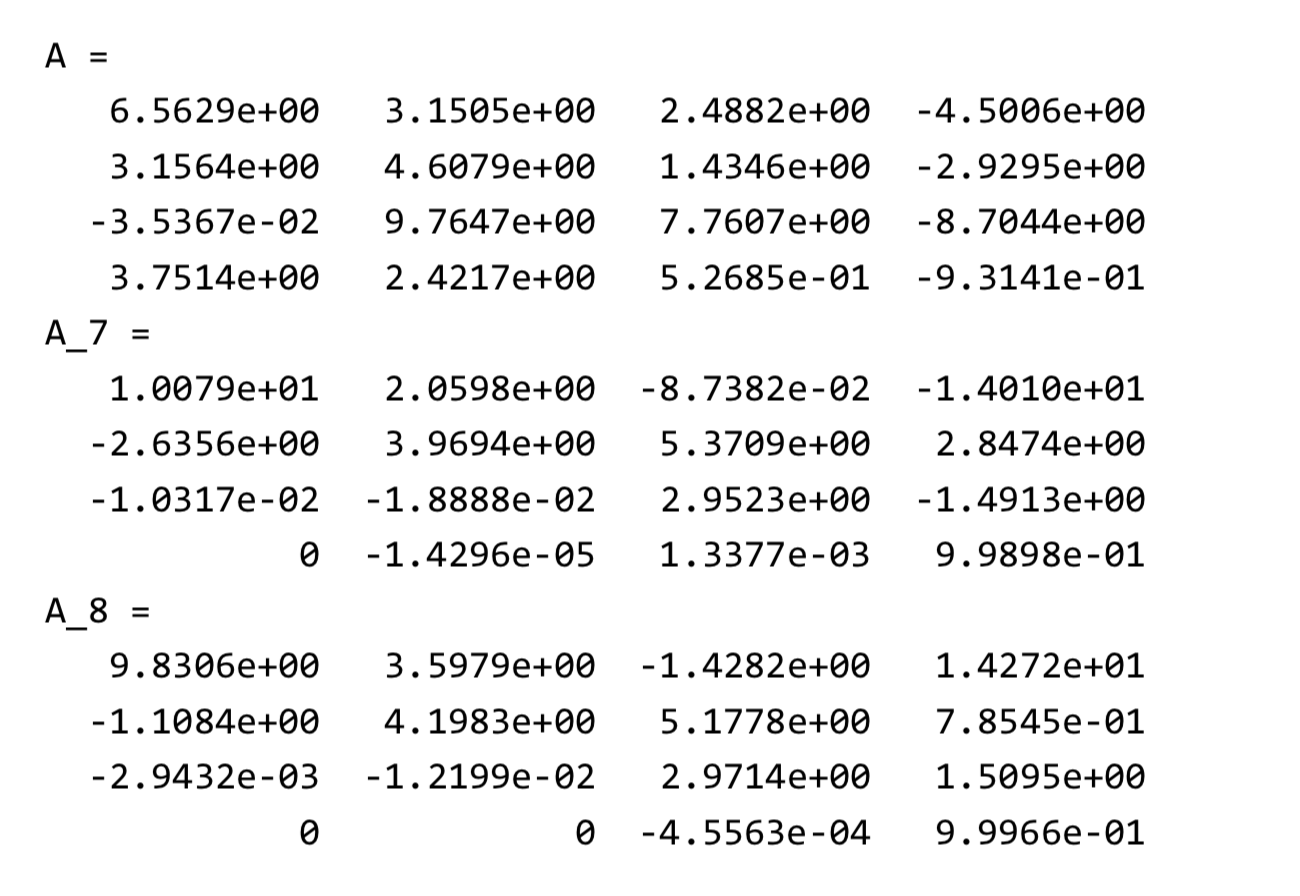
\includegraphics[scale=0.6]{figure4.png}
			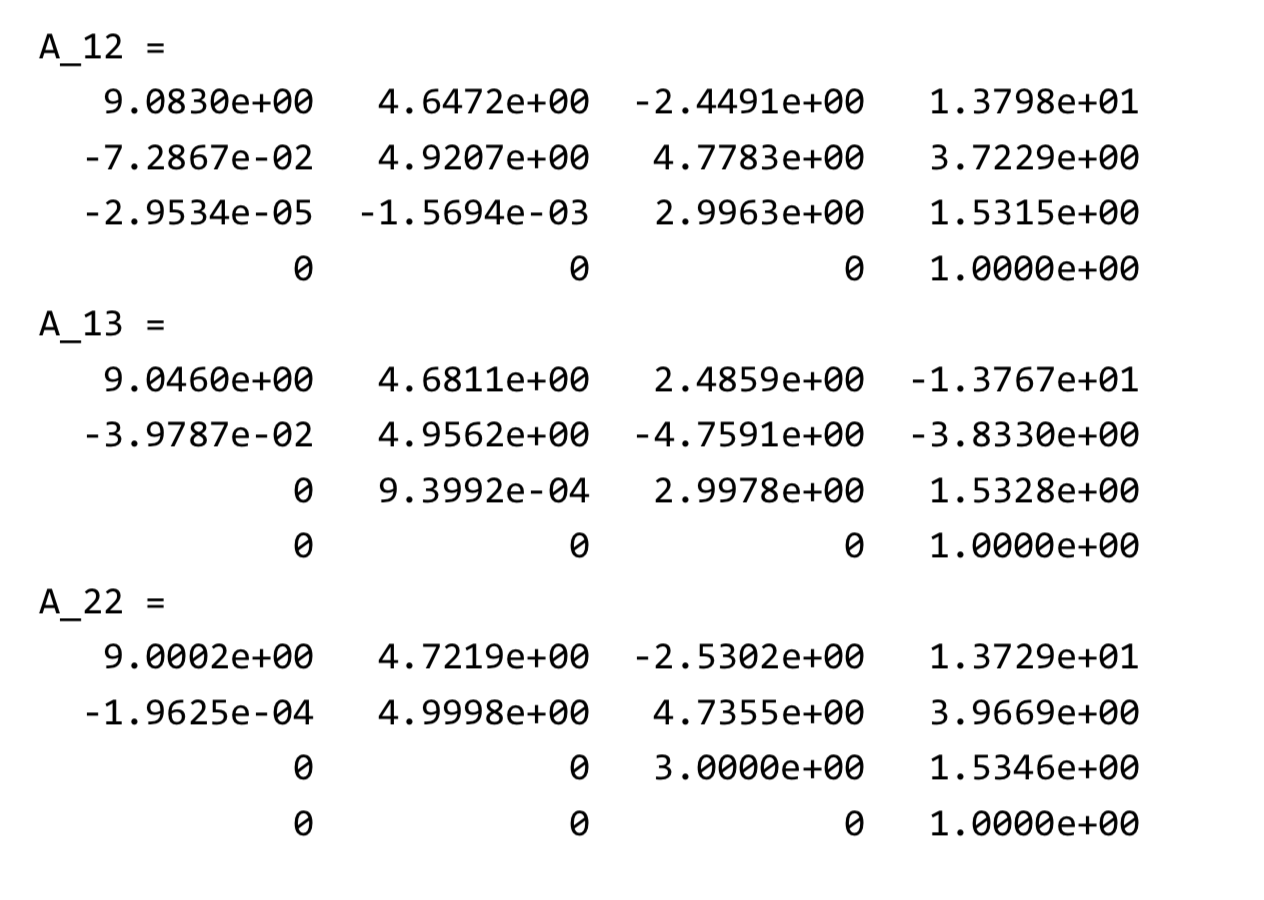
\includegraphics[scale=0.6]{figure5.png}
			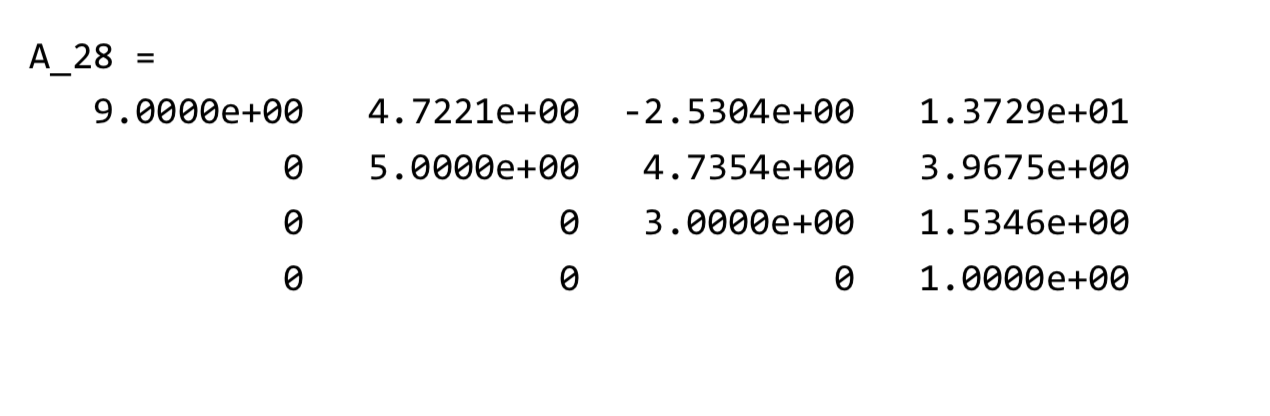
\includegraphics[scale=0.6]{figure6.png}
		\end{center}
	\end{figure}
	\newpage
	\subsubsection{带位移的QR迭代}
	为了加快 QR 迭代的收敛速度, 可以采用\textcolor{blue}{位移策略} 和\textcolor{blue}{反迭代}的思想\\
	\textcolor{blue}{算法 4.2} 带位移的QR 迭代算法 (QR Iteration with shift)\\
	\begin{enumerate}[1:]
		\item Set $A_{1}=A$ and $k=1$
		\item while not convergence do
		\item Choose a shift $\sigma_{k}$
		\item \qquad $[Q_{k},R_{k}]=qr(A_{k}-\sigma_{k}I)$
		\item \qquad compute $A_{k+1}=R_{k}Q_{k}+\sigma_{k}I$
		\item \qquad$k=k+1$
		\item end while
	\end{enumerate}
	正交相似性\\
	$$
	\begin{aligned} A_{k+1}=R_{k} Q_{k}+\sigma_{k} I &=\left(Q_{k}^{\top} Q_{k}\right) R_{k} Q_{k}+\sigma_{k} I \\ &=Q_{k}^{\top}\left(A_{k}-\sigma_{k} I\right) Q_{k}+\sigma_{k} I \\ &=Q_{k}^{\top} A_{k} Q_{k} \end{aligned}
	$$
	位移$\sigma_{k}$的选取\\
	在前面的分析可知,$A_{k+1}(n, n)$收敛到 A 的模最小特征值.\\
	若$\sigma_{k}$就是A的一个特征值,则$A_{k}-\sigma_{k} I$的模最小特征值为0,故QR算 法迭代一步就收敛. 此时
	$$
	A_{k+1}=R_{k} Q_{k}+\sigma_{k} I=\left[\begin{array}{cc}
	{A_{k+1}^{(n-1) \times(n-1)}} & {*} \\
	{0} & {\sigma_{k}}
	\end{array}\right]
	$$
	A 的其它特征值可通过对$A_{k+1}^{(n-1) \times(n-1)}$使用带位移 QR 迭代算法得到.\\
	通常, 如果 $\sigma_{k}$ 与 A 的某个特征值非常接近, 则收敛速度通常会很快. 由 于 $A_{k} (n, n)$ 收敛到 A 的一个特征值, 所以在实际使用中, 一个比较直观 的位移选择策略是$\sigma_{k} =A_{k}(n,n)$.事实上,这样的位移选取方法通常会 使得 QR 迭代算法有二次收敛速度.\\
	\\
	\textcolor{blue}{例}~带位移的 QR 迭代算法演示 $(见 Eig_QR_shift.m).$\\
	所有数据和设置与例 4.1 相同, 在迭代过程中, 取$\sigma_{k}=A_{k}(n, n)$.如果$A_{k}(n, n)$已经收敛, 则取$\sigma_{k}=A_{k}(n-1, n-1)$
	\begin{figure}
		\begin{center}
			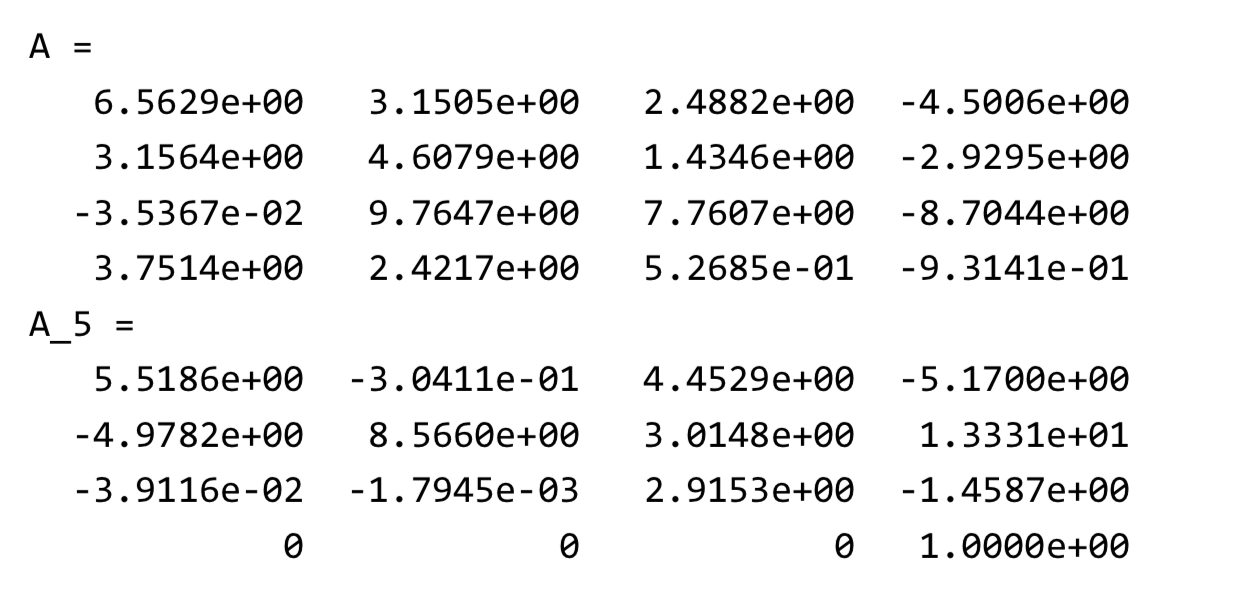
\includegraphics[scale=0.6]{figure7.png}
			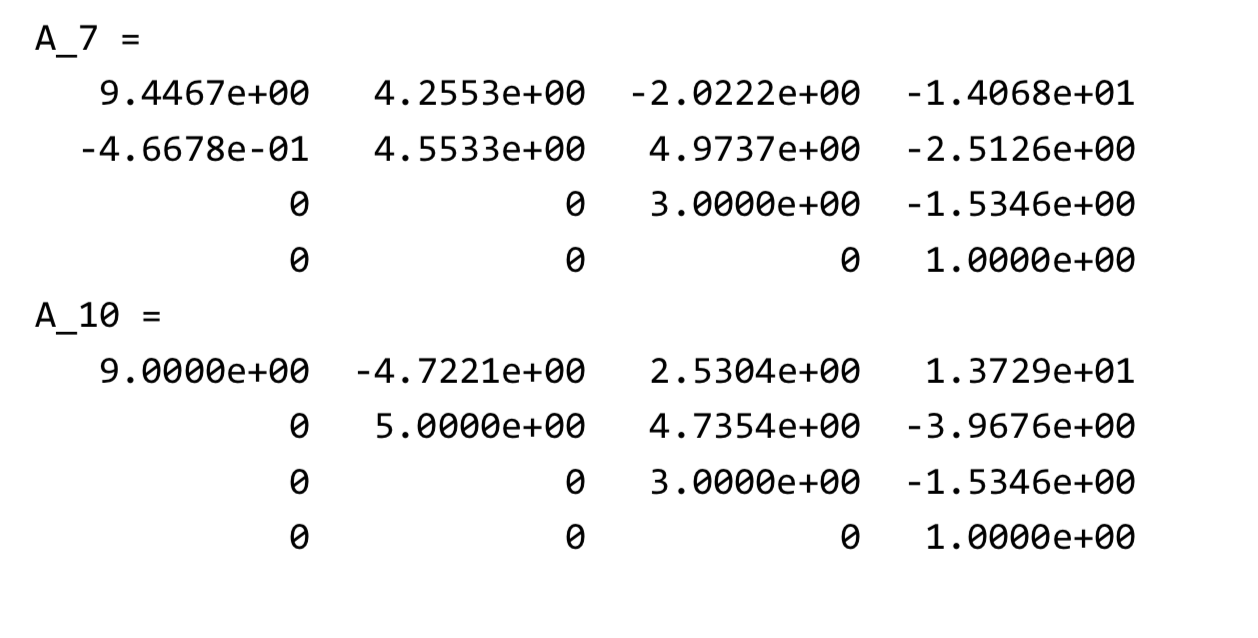
\includegraphics[scale=0.6]{figure8.png}
		\end{center}
	\end{figure}
	\subsection{带位移的隐式QR迭代}
	\noindent \textcolor{blue}{直接实施 QR 方法的困难: 运算量}\\
	每一步迭代需要做一次 QR 分解和矩阵乘积, 运算量为 $O\left(n^{3}\right)$ 即使每 计算一个特征值只需迭代一步, 则总运算量为$O\left(n^{4}\right)$\\
	我们的目标: 从$O\left(n^{4}\right)$减小到$O\left(n^{3}\right)$\\
	实现方法:两个步骤\\
	\begin{enumerate}[(1)]
		\item 首先通过相似变化将 A 转化成一个 上H
		essenberg 矩阵
		\item 对这个 Hessenberg 矩阵实施 隐式 QR 迭代
	\end{enumerate}
	\textcolor{blue}{隐式 QR 迭代}:\\
	在 QR 迭代算法中, 并 不进行显式的 QR 分解和矩阵乘积 , 而是通过 特殊手段 来实现从$A_{k}$到$A_{k+1}$的迭代,并且将运算量控制在$O\left(n^{2}\right)$量级,从而将总运算量降到$O(n^{3})$
	\subsubsection{上 Hessenberg 矩阵}
	\noindent \textcolor{blue}{上Hessenberg矩阵:}$H=\left[h_{i j}\right] \in \mathbb{R}^{n \times n}$当$i>j+1$时,有$h_{i j}=0$\\
	\textcolor{blue}{定理}设$A \in \mathbb{R}^{n \times n}$,则存在正交矩阵$Q \in \mathbb{R}^{n \times n}$使得$Q A Q^{\top}$是上Hessenberg矩阵\\
	下面我们以一个 $5\times 5$ 的矩阵 A 为例, 给出具体的转化过程, 采用的工具 为 Householder 变换.\\
	\textcolor{blue}{第一步}:令$Q_{1}=\operatorname{diag}\left(I_{1 \times 1}, H_{1}\right)$,其中$H_{1}$是对应于向量$A(2 : 5,1)$的 Householder 矩阵. 于是可得
	$$
	Q_{1} A=\left[\begin{array}{ccccc}
	* &*& *& *&* \\ 
	* &*& *& *&* \\ 
	0 &*& *& *&*\\ 
	0 &*& *& *&*\\ 
	0 &*& *& *&*
	\end{array}\right]
	$$
	由于用$Q_{1}^{T}$右乘$Q_{1} A$,不会改变$Q_{1} A$的第一列元素的值,故
	$$
	A_{1} \triangleq Q_{1} A Q_{1}^{\top}=\left[\begin{array}{ccccc}
	* &*& *& *&* \\ 
	* &*& *& *&* \\ 
	0 &*& *& *&*\\ 
	0 &*& *& *&*\\ 
	0 &*& *& *&*
	\end{array}\right]
	$$
	\textcolor{blue}{第二步}:令$Q_{2}=\operatorname{diag}\left(I_{2 \times 2}, H_{2}\right)$,其中$H_{2}$是对应于向量$A_{1}(3 : 5,2)$的 Householder 矩阵, 则用 $Q_{2}$ 左乘 $A_{1} $时, 不会改变 $A_{1}$ 的第一列元素 的值. 用$Q_{2}^{\top}$右乘$Q_{2} A_{1}$时,不会改变$Q_{2} A_{1}$前两列元素的值.因此
	$$
	Q_{2} A_{1}=\left[\begin{array}{ccccc}
	* &*& *& *&* \\ 
	* &*& *& *&* \\ 
	0 &*& *& *&*\\ 
	0 &0& *& *&*\\ 
	0 &0& *& *&*
	\end{array}\right]和
	A_{2}\triangleq Q_{2} A_{1} Q_{2}^{\top}=\left[\begin{array}{ccccc}
	* &*& *& *&* \\ 
	* &*& *& *&* \\ 
	0 &*& *& *&*\\ 
	0 &0& *& *&*\\ 
	0 &0& *& *&*
	\end{array}\right]
	$$
	\textcolor{blue}{第三步}:
	令$Q_{3}=\operatorname{diag}\left(I_{3 \times 3}, H_{3}\right)$,其中$H_{3}$是对应于向量$A_{2}(4 : 5,3)$的Householder 矩阵, 则有
	$$
	Q_{3} A_{2}=\left[\begin{array}{ccccc}
	* &*& *& *&* \\ 
	* &*& *& *&* \\ 
	0 &*& *& *&*\\ 
	0 &0& *& *&*\\ 
	0 &0& 0& *&*
	\end{array}\right]和A_{3} \triangleq Q_{3} A_{2} Q_{3}^{\top}=\left[\begin{array}{ccccc}
	* &*& *& *&* \\ 
	* &*& *& *&* \\ 
	0 &*& *& *&*\\ 
	0 &0& *& *&*\\ 
	0 &0& 0& *&*
	\end{array}\right]
	$$
	这时我们就将A转化成一个上Hessenberg矩阵,即
	$Q A Q^{\top}=A_{3}$,其中$Q=Q_{3} Q_{2} Q_{1}$是正交矩阵,$A_{3}$是上Hessenberg矩阵.

\textcolor{blue}{第三步:}\quad 令$Q_{3}=\operatorname{diag}\left(I_{3 \times 3}, H_{3}\right)$,其中$H_3$是对应于向量$A_2(4:5,3)$的Householder矩阵,则有$$
Q_{3} A_{2}=\left[\begin{array}{ccccc}{*} & {*} &{*} &{*} & {*} \\ {*} & {*} &{*} &{*} & {*} \\ {0} & {*} &{*} & {*} &{*} \\ {0} & {0} & {*} &{*} & {*} \\ {0} & {0} & {0} & {*} &{*}\end{array}\right]
\text{和} A_{3} \triangleq Q_{3} A_{2} Q_{3}^{\top}=\left[\begin{array}{ccccc}{*} & {*} &{*} &{*} & {*} \\ {*} & {*} &{*} &{*} & {*} \\ {0} & {*} &{*} &{*} & {*} \\  {0} & {0} & {*} &{*} & {*} \\ {0} & {0} & {0} &{*} & {*}\end{array}\right]
$$
这时,我们就将$A$转化成一个上Hessenberg矩阵,即$QAQ^T=A_3$,其中$Q=Q_3Q_2Q_1$是正交矩阵,$A_3$是上Hessenberg矩阵。

上Hessenberg化算法\\
\textcolor{blue}{算法 5.1}\quad 上Hessenberg化算法(Upper Hessenberg Reduction)
\begin{enumerate}[1:]
	\item set $Q=I$
	\item for $k=1$ to $n-2$ do
	\item \quad compute Hessenberg matrix $H_k$ with respect to $A(k+1:n,k)$
	\item \quad $\begin{aligned} A(k+1& : n, k : n )=H_{k} \cdot A(k+1 : n, k : n) \\ &=A(k+1 : n, k : n)-\beta_{k} v_{k}\left(v_{k}^{\top} A(k+1 : n, k : n)\right) \end{aligned}$
	\item \quad $\begin{aligned} A(1 : n, &k+1 : n)=A(1 : n, k+1 : n) \cdot H_{k}^{\top}\\
	&=A(1 : n, k+1 : n)-\beta_{k} A(1 : n, k+1 : n) v_{k} v_{k}^{\top} \end{aligned}$
	\item \quad $\begin{aligned} Q(k+1& : n, k : n )=H_{k} \cdot Q(k+1 : n, k : n) \\ &=Q(k+1 : n, k : n)-\beta_{k} v_{k}\left(v_{k}^{\top} Q(k+1 : n, k : n)\right) \end{aligned}$
	\item end for
\end{enumerate}

\textcolor{blue}{说明:}
\begin{itemize}
	\item 在实际计算时,我们不需要显式地形成Householder矩阵$H_k$。
	\item 上述算法的运算量大约为$\frac{14}{3} n^{3}+\mathcal{O}\left(n^{2}\right)$。如果不需要计算特征向量,则正交矩阵$Q$也不用计算,此时运算量大约为$\frac{10}{3} n^{3}+\mathcal{O}\left(n^{2}\right)$。
	\item 上Hessenberg矩阵的一个很重要的性质就是在QR迭代中保持形状不变。
\end{itemize}

\textcolor{blue}{定理}\quad 设$A \in \mathbb{R}^{n \times n}$是非奇异上Hessenberg矩阵,其QR分解为$A=QR$,则$\tilde{A} \triangleq R Q$也是上Hessenberg矩阵。

若$A$是奇异的,也可以通过选取适当的$Q$,使得上述结论成立。

由此可知,如果$A$是上Hessenberg矩阵,则QR迭代中的每一个$A_k$都是上Hessenberg矩阵矩阵。这样在进行QR分解时,运算量可大大降低。

Hessenberg矩阵另一重要性质:在QR迭代中保持下次对角线元素非零。

\textcolor{blue}{定理}\quad 设$A \in \mathbb{R}^{n \times n}$是上Hessenberg矩阵且下次对角线元素均非零,即$a_{i+1, i} \neq 0, i=1,2, \ldots, n-1$。设其QR分解为$A=QR$,则$\tilde{A} \triangleq R Q$的下次对角线元素也都非零。

若$A$村咋子某个下次对角线元素为零,则$A$一定可约。因此,我们只需考虑下次对角线均非零的情形。

\textcolor{blue}{推论}\quad $\tilde{A} \triangleq R Q$则在带位移的QR迭代中,所有的$A_k$的下次对角线元素均非零。
\subsubsection{隐式QR迭代}
在QR迭代中,我们要先做QR分解$A_k=Q_kR_k$,然后计算$A_{k+1}k=Q_kR_k$.但事实上,我们可以直接计算出$A_{k+1}$。这就是\textcolor{blue}{隐式QR迭代}。

不失一般性,我们假定$A$是不可约的上Hessenberg矩阵。

隐式QR迭代的理论基础就是下面的\textcolor{blue}{隐式Q定理}。

\textcolor{blue}{定理(ImplicitQTheorem)}\quad 设$H=Q^{\top} A Q \in \mathbb{R}^{n \times n}$是一个不可约上Hessenberg矩阵,其中$Q \in \mathbb{R}^{n \times n}$是正交矩阵,则$Q$的第$2$至第$n$列均由$Q$的第一列所唯一确定(可相差一个符号)。

由于$Q_k$的其他列都由$Q_k$的第一列唯一确定(至多相差一个符号),所以我们只要找到一个正交矩阵$\tilde{Q}_{k}$使得其第一列与$\tilde{Q}_{k}$的第一列相等,且$\tilde{Q}_{k}^{\top} A_{k} \tilde{Q}_{k}$为上Hessenberg矩阵,则由隐式$Q$定理可知$\tilde{Q}_{k}=W Q_{k}$,其中$W=\operatorname{diag}(1, \pm 1, \ldots, \pm 1)$,于是$$
\tilde{Q}_{k}^{\top} A_{k} \tilde{Q}_{k}=W^{\top} Q_{k}^{\top} A_{k} Q_{k} W=W^{\top} A_{k+1} W
$$。
又$W^{\top} A_{k+1} W$与$A_{k+1}$相似,且对角线元素相等,而其他元素也至多相差一个符号,所以不会影响$A_{k+1}$的收敛性,即下三角元素收敛到$0$,对角线元素收敛到$A$的特征值。

在QR迭代算法中,如果我们直接令$A_{k+1}=\tilde{Q}_{k}^{\top} A_{k} \tilde{Q}_{k}$,则其收敛性与原QR迭代算法没有任何区别!这就是隐式QR迭代的基本思想。

由于$A$是上Hessenberg矩阵,因此在实际计算中,我们只需Givens变换。

下面我们举一个例子,具体说明如何利用隐式Q定理,由$A_1$得到$A_2$。

设$A \in \mathbb{R}^{5 \times 5}$是一个不可约上Hessenberg矩阵,即$$
A_{1}=A=\left[\begin{array}{ccccc}{*} & {*} & {*}& {*}& {*} \\ {*} & {*} & {*}& {*}& {*} \\ {0} & {*} & {*}& {*}& {*} \\ {0} & {0} & {*} & {*}& {*} \\ {0} & {0} & {0} & {*}& {*}\end{array}\right]
$$
\textcolor{blue}{第一步:}\quad 构造一个Givens变换
$$
G_{1}^{\top} \triangleq G\left(1,2, \theta_{1}\right)=\left[\begin{array}{ccc}{c_{1}} & {s_{1}}& \\ {-s_{1}} & {c_{1}} &\\ {} && {I_{3}}\end{array}\right]
\qquad (c_1,s_1\text{待定})
$$
于是有$$
G_{1}^{\top} A=\left[\begin{array}{ccccc}{*}  & {*} & {*}& {*}& {*}\\ {*} & {*} & {*} & {*}& {*}\\ {0} & {*} & {*}& {*}& {*} \\ {0} & {0} & {*} & {*}& {*}\\ {0} & {0} & {0} & { *}& {*}\end{array}\right] \text{和}A^{(1)} \triangleq G_{1}^{\top} A G_{1}=\left[\begin{array}{ccccc}{*}  & {*} & {*}& {*} & {*} \\ {*}  & {*} & {*}& {*} & {*} \\ {+} & {*} & {*}  & {*} & {*}\\ {0} & {0} & {*} & {*}  & {*}\\ {0} & {0} & {0} & {*} & {*}\end{array}\right]
$$
与$A_1$相比较,$A^{(1)}$在$(3,1)$位置上多出一个非零元,我们把它记为“+”,并称之为\textcolor{blue}{bulge}。在下面的计算过程中,我们的目标就是将其“赶”出矩阵,从而得到一个新的上Hessenberg矩阵,即$A_2$。

\textcolor{blue}{第二步:}\quad 为了消去这个bulge,我们可以构造Givens变换$$
G_{2}^{\top} \triangleq G\left(2,3, \theta_{2}\right)=\left[\begin{array}{cccc}{1} & {} & {} &\\ {} & {c_{2}} & {s_{2}}& \\ {} & {-s_{2}} & {c_{2}} &\\ {} & {} && {I_{2}}\end{array}\right]
\text{使得}G_{2}^{\top} A^{(1)}=\left[\begin{array}{ccccc}{*} & {*} & {*} & {*}& {*}\\ {*} & {*} & {*} & {*} & {*}\\ {0} & {*} & {*} & {*}& {*} \\ {0} & {0} & {*} & {*}& {*} \\ {0} & {0} & {0} & {*}& {*}\end{array}\right]$$

为了保持与原矩阵的相似性,需要再右乘$G_2$,所以$$
A^{(2)} \triangleq G_{2}^{\top} A^{(1)} G_{2}=\left[\begin{array}{ccccc}{*} & {*} & {*} & {*}& {*}\\ {*} & {*} & {*} & {*}& {*}\\ {0} & {*} & {*}& {*}& {*} \\ {0} & {+} & {*} & {*}& {*}\\ {0} & {0} & {0} & {*}& {*}\end{array}\right]
$$
此时,bugle从$(3,1)$位置被“赶”到$(4,2)$位置。

\textcolor{blue}{第三步:}\quad 与第二步类似,构造Givens变换$$
G_{3}^{\top} \triangleq G\left(3,4, \theta_{3}\right)=\left[\begin{array}{cccc}{I_{2}} & {} & {}& {} \\ {} & {c_{3}} & {s_{3}} & {}\\ {} & {-s_{3}}& { c_{3}} & {}\\ {} & {}& {} & {1}\end{array}\right]
\text{使得}G_{3}^{\top} A^{(2)}=\left[\begin{array}{ccccc}{*} & {*} & {*} & {*}& {*}\\ {*} & {*} & {*} & {*} & {*}\\ {0} & {*} & {*} & {*}& {*} \\ {0} & {0} & {*} & {*}& {*} \\ {0} & {0} & {0} & {*}& {*}\end{array}\right]
$$这时$$
A^{(3)} \triangleq G_{3}^{\top} A^{(2)} G_{3}=\left[\begin{array}{ccccc}{*} & {*} & {*} & {*}& {*}\\ {*} & {*} & {*} & {*}& {*}\\ {0} & {*} & {*}& {*}& {*} \\ {0} & {0} & {*} & {*}& {*}\\ {0} & {0} & {+} & {*}& {*}\end{array}\right]
$$
于是,bugle又从$(4,2)$位置被“赶”到$(5,3)$位置。

\textcolor{blue}{第四步:}\quad 再次构造Givens变换$$
G_{4}^{\top} \triangleq G\left(4,5, \theta_{4}\right)=\left[\begin{array}{ccccc}{1} & {} & {}& {} &\\ {} & {1} & {} & {}&\\ {} & {}& {1} & {}&\\ {} & {}& {} & {c_4}&s_4\\{} & {}& {} & {-s_4}&c_4\end{array}\right]
\text{使得}G_{4}^{\top} A^{(3)}=\left[\begin{array}{ccccc}{*} & {*} & {*} & {*}& {*}\\ {*} & {*} & {*} & {*} & {*}\\ {0} & {*} & {*} & {*}& {*} \\ {0} & {0} & {*} & {*}& {*} \\ {0} & {0} & {0} & {*}& {*}\end{array}\right]
$$这时$$
A^{(4)} \triangleq G_{4}^{\top} A^{(3)} G_{4}=\left[\begin{array}{ccccc}{*} & {*} & {*} & {*}& {*}\\ {*} & {*} & {*} & {*}& {*}\\ {0} & {*} & {*}& {*}& {*} \\ {0} & {0} & {*} & {*}& {*}\\ {0} & {0} & {0} & {*}& {*}\end{array}\right]
$$
现在,bulge被“赶”出矩阵,$A{(4)}$就是我们所要的矩阵!\\
\textbf{算法分析,以及$c_1,s_1$的取值}

常规QR迭代:$A_{1}=Q_{1} R_{1}, A_{2}=R_{1} Q_{1} \Longrightarrow A_{2}=Q_{1}^{\top} A_{1} Q_{1}$

根据前面的计算过程,有$$
A^{(4)}=G_{4}^{\top} G_{3}^{\top} G_{2}^{\top} G_{1}^{\top} A_{1} G_{1} G_{2} G_{3} G_{4}=\tilde{Q}_{1}^{\top} A_{1} \tilde{Q}_{1}
$$,其中$\tilde{Q}_{1}=G_{1} G_{2} G_{3} G_{4} \Longrightarrow A^{(4)}=\tilde{Q}_{1}^{\top} A_{1} \tilde{Q}_{1}$

通过直接计算可知,$\tilde{Q}_{1}$的第一列为$$
\left[c_{1}, s_{1}, 0,0,0\right]^{\top}
$$

如果将其取为$A_1$的第一列$\left[a_{11}, a_{21}, 0, \ldots, 0\right]^{\top}$单位化后的向量,\textcolor{blue}{则$\tilde{Q}_{1}$的第一列与$Q_{1}$的第一列相同!$\Longrightarrow A^{(4)}=W^{\top} A_{2} W$}

针对带位移的QR方法,我们取$A_{1}-\sigma_{1} I$的第一列$$
\left[a_{11}-\sigma_{1}, a_{21}, 0, \ldots, 0\right]^{\top}
$$单位化后的向量作为$G_1$的第一列即可。\\
\textcolor{blue}{运算量:}

如果$A \in \mathbb{R}^{n \times n}$是上Hessenberg矩阵,则使用上面的算法,带位移QR迭代中每一步的运算量为$6 n^{2}+O(n)$。

\subsubsection{位移的选取}
通常,位移越离某个特征值越近,则收敛速度就越快。

由习题4.10可知,如果位移$\sigma$与某个特征值非常接近,则$A_{k}(n, n)-\sigma$就非常接近于0。

这说明\textcolor{blue}{$A_k(n,n)$通常会首先收敛到$A$的一个特征值。}所以\textcolor{blue}{$\sigma=A_{k}(n, n)$是一个不错的选择。}但是,如果这个特征值是复数,这种唯一选取方法就可能失效。

\textbf{双位移策略}

设$\sigma \in \mathbb{C}$是$A$的某个复特征值$\lambda$的一个很好的近似,则其共轭$\overline{\sigma}$也应该是$\overline{\lambda}$的一个很好的近似。因此我们可以考虑\textcolor{blue}{双位移}策略,即先以$\lambda$为位移迭代一次,然后再以$\overline{\sigma}$为位移迭代一次,如此不断交替进行迭代。

这样就有$$
\begin{aligned} A_{1}-\sigma I &=Q_{1} R_{1} \\ A_{2} &=R_{1} Q_{1}+\sigma I \\ A_{2}-\overline{\sigma} I &=Q_{2} R_{2} \\ A_{3} &=R_{2} Q_{2}+\overline{\sigma} I \end{aligned}
$$容易验证$$
A_{3}=Q_{2}^{\top} A_{2} Q_{2}=Q_{2}^{*} Q_{1}^{*} A_{1} Q_{1} Q_{2}=Q^{*} A_{1} Q
$$其中$Q=Q_1Q_2$

我们注意到$\sigma$可能是复的,所以$Q_1$和$Q_2$都可能是复矩阵。但我们却可以选取适当的$Q_1$和$Q_2$,使得$Q=Q_1Q_2$是实矩阵。

\textbf{双位移策略的实现}

由前面的结论可知,存在$Q_1$和$Q_2$,使得$Q=Q_1Q_2$是实矩阵,从而$$
A_{3}=Q^{\top} A_{1} Q
$$也是实矩阵。因此我们希望\textcolor{blue}{不计算$A_2$,而是直接从$A_1$得到$A_3$}\\
\textcolor{blue}{实现方式:}

根据隐式Q定理:只要找到一个实正交矩阵$Q$,使得其第一列与$$
A_{1}^{2}-2 \operatorname{Re}(\sigma) A_{1}+|\sigma|^{2} I
$$的第一列平行,并且$A_{3}=Q^{\top} A_{1} Q$是上Hessenberg矩阵即可。

易知,$A_{1}^{2}-2 \operatorname{Re}(\sigma) A_{1}+|\sigma|^{2} I$的第一列为\begin{equation}
\left[\begin{array}{c}{a_{11}^{2}+a_{12} a_{21}-2 \operatorname{Re}(\sigma) a_{11}+|\sigma|^{2}} \\ {a_{21}\left(a_{11}+a_{22}-2 \operatorname{Re}(\sigma)\right)} \\ {a_{21} a_{32}} \\ {0} \\ {\vdots}\end{array}\right]
\end{equation}
所以$Q$的第一列是上述向量的单位化。

其他过程可以通过隐式QR迭代来实现。但此时的“bulge"是一个$2\times 2$的小矩阵。因此,在双位移隐式R迭代过程中,\textcolor{blue}{需要使用Householder变换。}

需要指出的是,\textcolor{blue}{双位移QR迭代算法中的运算都是实数运算。}

下面通过一个例子来说明如何在实数运算下实现双位移隐式QR迭代。

设$A \in \mathbb{R}^{6 \times 6}$是一个不可约上Hessenberg矩阵,即$$
A_{1}=A=\left[\begin{array}{cccccc}{*} & {*} & {*}  & {*} & {*} & {*}\\ {*} & {*} & {*} & {*} & {*} & {*} \\ {0} & {*} & {*} & {*}  & {*} & {*}\\ {0} & {0} & {*} & {*} & {*} & {*} \\ {0}& {0}  & {0} & {*} & {*}  & {*} \\ {0} & {0} & {0} & {0} & {*} & {*}\end{array}\right]
$$

\textcolor{blue}{第一步:}\quad 构造一个正交矩阵$H_{1}=\left[\begin{array}{cc}{\tilde{H}_{1}^{\top}} & {0} \\ {0} & {I_{3}}\end{array}\right]$,其中$\tilde{H}_{1} \in \mathbb{R}^{3 \times 3}$,使得第一列与$A_{1}^{2}-2 \operatorname{Re}(\sigma) A_{1}+|\sigma|^{2} I$的第一列平行。于是有$$
H_{1}^{\top} A=\left[\begin{array}{cccccc}{*} & {*} & {*} & {*} & {*}& {*}\\ {*} & {*} & {*} & {*}& {*}& {*} \\ {+} & {*} & {*} & {*}& {*}& {*} \\ {0} & {0} & {*} & {*}& {*}& {*} \\ {0} & {0} & {0} & {*} & {*}& {*}\\ {0} & {0} & {0} & {0} & {*}& {*}\end{array}\right]
\text{和}A^{(1)} \triangleq H_{1}^{\top} A H_{1}=\left[\begin{array}{cccccc}{*} & {*} & {*} & {*}& {*}& {*} \\ {*} & {*} & {*} & {*}& {*}& {*} \\ {+} & {*} & {*} & {*}& {*}& {*} \\ {+} & {+} & {*}& {*} & {*} & {*}  \\ {0} & {0} & {0} & {*} & {*}& {*} \\ {0} & {0} & {0} & {0 }& {*}& {*}\end{array}\right]
$$
与$A_1$相比较,$A^{(1)}$在$(3,1),(4,1)$和$(4,2)$位置上出现bulge。在下面的计算过程中,我们的目标就是把它们”赶“出矩阵,从而得到一个新的上Hessenberg矩阵。

\textcolor{blue}{第二步:}\quad 令$H_{2}=\left[\begin{array}{ccc}{1} & {0} & {0} \\ {0} & {\tilde{H}_{2}^{\top}} & {0} \\ {0} & {0} & {I_{2}}\end{array}\right]$,其中$\tilde{H}_{2} \in \mathbb{R}^{3 \times 3}$是对应于$A(2 : 4,1)$的Householder变换,使得$$
H_{2}^{\top} A^{(1)}=\left[\begin{array}{cccccc}{*} & {*} & {*}& {*}& {*}& {*} \\ {*} & {*} & {*} & {*}& {*}& {*}\\ {0} & {*} & {*} & {*} & {*}& {*}\\ {0} & {+} & {*} & {*}& {*}& {*}\\ {0} & {0} & {0} & {*}& {*}& {*}\\ {0} & {0} & {0} & {0}& {*}& {*}\end{array}\right]
\text{和}A^{(2)} \triangleq H_{2}^{\top} A^{(1)} H_{2}=\left[\begin{array}{cccccc}{*} & {*} & {*}& {*}& {*}& {*} \\ {*} & {*} & {*} & {*}& {*}& {*}\\ {0} & {*} & {*} & {*} & {*}& {*}\\ {0} & {+} & {*} & {*}& {*}& {*}\\ {0} & {+} & {+} & {*}& {*}& {*}\\ {0} & {0} & {0} & {0}& {*}& {*}\end{array}\right]
$$
这时,我们将bugle向右下角方向”赶“了一个位置。

\textcolor{blue}{第三步}\quad 与第二步类似,令$H_{3}=\left[\begin{array}{ccc}{I_2} & {0} & {0} \\ {0} & {\tilde{H}_{3}^{\top}} & {0} \\ {0} & {0} & {1}\end{array}\right]$,其中$\tilde{H}_{3} \in \mathbb{R}^{3 \times 3}$是对应于$A(3 : 5,2)$的Householder变换,使得$$
H_{3}^{\top} A^{(2)}=\left[\begin{array}{cccccc}{*} & {*} & {*}& {*}& {*}& {*} \\ {*} & {*} & {*} & {*}& {*}& {*}\\ {0} & {*} & {*} & {*} & {*}& {*}\\ {0} & {0} & {*} & {*}& {*}& {*}\\ {0} & {0} & {+} & {*}& {*}& {*}\\ {0} & {0} & {0} & {0}& {*}& {*}\end{array}\right]
\text{和}A^{(3)} \triangleq H_{3}^{\top} A^{(2)} H_{3}=\left[\begin{array}{cccccc}{*} & {*} & {*}& {*}& {*}& {*} \\ {*} & {*} & {*} & {*}& {*}& {*}\\ {0} & {*} & {*} & {*} & {*}& {*}\\ {0} & {0} & {*} & {*}& {*}& {*}\\ {0} & {0} & {+} & {*}& {*}& {*}\\ {0} & {0} & {+} & {+}& {*}& {*}\end{array}\right]
$$
这时,bugle又被向右下角方向”赶“了一个位置。

\textcolor{blue}{第四步}\quad 令$H_{4}=\left[\begin{array}{cc}{I_3} & {0} \\ {0} & {\tilde{H}_{4}^{\top}}  \end{array}\right]$,其中$\tilde{H}_{4} \in \mathbb{R}^{3 \times 3}$是对应于$A(4: 6,3)$的Householder变换,使得$$
H_{4}^{\top} A^{(3)}=\left[\begin{array}{cccccc}{*} & {*} & {*}& {*}& {*}& {*} \\ {*} & {*} & {*} & {*}& {*}& {*}\\ {0} & {*} & {*} & {*} & {*}& {*}\\ {0} & {0} & {*} & {*}& {*}& {*}\\ {0} & {0} & {0} & {*}& {*}& {*}\\ {0} & {0} & {0} & {+}& {*}& {*}\end{array}\right]
\text{和}A^{(4)} \triangleq H_{4}^{\top} A^{(3)} H_{4}=\left[\begin{array}{cccccc}{*} & {*} & {*}& {*}& {*}& {*} \\ {*} & {*} & {*} & {*}& {*}& {*}\\ {0} & {*} & {*} & {*} & {*}& {*}\\ {0} & {0} & {*} & {*}& {*}& {*}\\ {0} & {0} & {0} & {*}& {*}& {*}\\ {0} & {0} & {0} & {+}& {*}& {*}\end{array}\right]
$$

\textcolor{blue}{第五步}\quad 只需构造一个Givens变换$G_{5}=\left[\begin{array}{cc}{I_4} & {0} \\ {0} & {G(4,5,\theta)^{\top}}  \end{array}\right]$,使得$$
G_{}5^{\top} A^{(4)}=\left[\begin{array}{cccccc}{*} & {*} & {*}& {*}& {*}& {*} \\ {*} & {*} & {*} & {*}& {*}& {*}\\ {0} & {*} & {*} & {*} & {*}& {*}\\ {0} & {0} & {*} & {*}& {*}& {*}\\ {0} & {0} & {0} & {*}& {*}& {*}\\ {0} & {0} & {0} & {0}& {*}& {*}\end{array}\right]
\text{和}A^{(5)} \triangleq G_{5}^{\top} A^{(4)} G_{5}=\left[\begin{array}{cccccc}{*} & {*} & {*}& {*}& {*}& {*} \\ {*} & {*} & {*} & {*}& {*}& {*}\\ {0} & {*} & {*} & {*} & {*}& {*}\\ {0} & {0} & {*} & {*}& {*}& {*}\\ {0} & {0} & {0} & {*}& {*}& {*}\\ {0} & {0} & {0} & {0}& {*}& {*}\end{array}\right]
$$

现在,bulge已经被全部消除,且$$A^{(5)}=Q^{\top} A Q$$,其中$Q=H_{1} H_{2} H_{3} H_{4} G_{5}$。通过直接计算可知,$Q$的第一列即为$H_1$的第一列。根据隐式Q定理,可以直接令$A_{3} \triangleq A^{(5)}=Q^{\top} A Q$。

\textbf{位移的具体选取}

在单位移QR迭代算法中,若$A$的特征值都是实的,则取$\sigma_{k}=A_{k}(n, n)$.推广到复共轭特征值上,我们可以取$A_k$的右下角矩阵$$
\left[\begin{array}{cc}{A_{k}(n-1, n-1)} & {A_{k}(n-1, n)} \\ {A_{k}(n, n-1)} & {A_{k}(n, n)}\end{array}\right]
$$的复共轭特征值作为双位移。这样选取的位移就是\textcolor{blue}{Francis位移}。

如果上述矩阵的两个特征值都是实的,则选取其中模较小的特征值做单位移。

采用Francis位移的QR迭代会使得$A_k$的右下角收敛到一个上三角矩阵(两个实特征值)或一个2阶的矩阵(一对复共轭特征值),而且通常会有二次收敛性。在实际计算中,一个特征值一般平均只需迭代两步。\\
\textcolor{blue}{收敛性判断:}

判断收敛性主要是看$A_{k}(n-1, n-2)$(或$A_{k}(n, n-1)$)是否趋向于$0$。

需要指出的是,QR迭代并不是对所有的矩阵都收敛。例如:$$A=\left[\begin{array}{lll}{0} & {0} & {1} \\ {1} & {0} & {0} \\ {0} & {1} & {0}\end{array}\right]$$
对于上面的矩阵,采用Francis位移的QR迭代算法无效。另外,也可以考虑多重位移策略,参见\textcolor{blue}{[Watkins 2007]}。
\subsubsection{收缩Deflation}
收缩(deflation)技术是实用QR迭代中的一个非常重要概念。

隐式QR迭代过程中,当矩阵$A_{k+1}$的某个下次对角线元素$a_{i+1}$,$i$很小时,我们可以将其设为$0$。

由于$A_{k+1}$是上Hessenberg矩阵,这时$A_{k+1}$就可以写成分块上三角形式,其中两个对角块都是上Hessenberg矩阵。

因此我们可以将隐式QR迭代作用在这两个规模相对较小的矩阵上,从而可以大大节约运算量。
\subsection{特征向量的计算}
设$A$的特征值都是实的,$R=Q^TAQ$是其Schur标准型。若$Ax=\lambda x$,则 $Ry=\lambda y$,其中$y=Q^Tx$或$x=Qy$。故只需计算R的特征向量$y$即可。

因为$R$的对角线元素即为$A$的特征值,不妨设$\lambda=R(i,i)$。

假定$\lambda$是单重特征值,则方程$(R-\lambda I)y=0$即为$$
\left[\begin{array}{ccc}{R_{11}-\lambda I R_{12}} & {R_{13}} \\ {0} & {0} & {R_{23}} \\ {0} & {0} & {R_{33}-\lambda I}\end{array}\right]\left[\begin{array}{l}{y_{1}} \\ {y_{2}} \\ {y_{3}}\end{array}\right]=0
$$即\begin{equation}
\left(R_{11}-\lambda I\right) y_{1}+R_{12} y_{2}+R_{13} y_{3}=0
\end{equation}\begin{equation}
R_{23} y_{3}=0
\end{equation}\begin{equation}
\left(R_{33}-\lambda I\right) y_{3}=0
\end{equation}其中$R_{11} \in \mathbb{R}^{(i-1) \times(i-1)}, R_{33} \in \mathbb{R}^{(n-i) \times(n-i)}$。由于$\lambda$是单重特征值,故
$R_{33}-\lambda I$非奇异,因此$y_3=0$。令$y_2=1$,则可得$$
y_{1}=\left(R_{11}-\lambda I\right)^{-1} R_{12}
$$

因此计算特征向量$y$只需求解一个上三角线性方程组。

若$\lambda$是多重特征值,则据算方法类似。但如果$A$有负特征值,则需要利用实Schur标准型,计算较复杂。
\subsection{广义特征值问题}
设$A, B \in \mathbb{R}^{n \times n}$,若存在$\lambda \in \mathbb{C}$和非零向量$x \in \mathbb{C}^{n}$使得$$
A x=\lambda B x
$$则称$\lambda$为矩阵对$(A,B)$的特征值,$x$为对应的特征向量。

计算矩阵对$(A,B)$的特征值和特征向量就是\textcolor{blue}{广义特征值问题}

当$B$非奇异时,广义特征值问题就等价于标准特征值问题$$
B^{-1} A x=\lambda x
 \text{或}A B^{-1} y=\lambda y
$$其中$y=Bx$。

容易看出,$\lambda$是$(A,B)$的一个特征值当且仅当\begin{equation}
\operatorname{det}(A-\lambda B)=0
\label{equation4.9}
\end{equation}

若\ref{equation4.9}对所有$\lambda \in \mathbb{C}$都成立,则称矩阵对$(A,B)$是\textcolor{blue}{奇异矩阵对},否则称为\textcolor{blue}{正则矩阵对}。

当$B$非奇异时,特征方程\ref{equation4.9}是一个$n$次多项式,因此恰好有$n$个特好找呢个字。当$B$奇异时,特征方程\ref{equation4.9}的次数低于$n$,因此方程的解的个数小于$n$。但是,注意带$\lambda \neq 0$是$(A,B)$的t特征值当且仅当$\mu=\frac{1}{\lambda}$是$(B, A)$的特征值。因此,当$B$奇异时,$\mu=0$是$(B, A)$的特征值,于是我们自然的把$\lambda=\frac{1}{u}=\infty$当作是$(A,B)$的特征值。所以广义特征值不是分布在$\mathbb{C}$上,而是分布在$\mathbb{C} \cup\{\infty\}$上。

容易验证,若$U,V$非奇异,则矩阵对$\left(U^{*} A V, U^{*} B V\right)$的特征值与$(A,B)$是一样的。因此我们称这种变换为\textcolor{blue}{矩阵对的等价变换}。如果$U,V$是酉矩阵,则称为\textcolor{blue}{酉等价变换}。
\subsubsection{广义Schur分解}
\textcolor{blue}{广义Schur分解}是矩阵对在酉等价变换下的最简形式。

\textcolor{blue}{定理(广义Schur分解)}\quad 设$A, B \in \mathbb{C}^{n \times n}$,则存在酉矩阵$Q, Z \in \mathbb{C}^{n \times n}$,使得\begin{equation}
Q^{*} A Z=R_{A}, \quad Q^{*} B Z=R_{B}
\end{equation}其中$R_{A}, R_{B} \in \mathbb{C}^{n \times n}$都是上三角矩阵。此时矩阵对$(A,B)$的特征值为$R_A$和$R_B$的对角线元素的比值,即$$
\lambda_{i}=\frac{R_{A}(i, i)}{R_{B}(i, i)}, \quad i=1,2, \ldots, n
$$当$R_{B}(i, i)=0$时,对应的特征值$\lambda_{i}=\infty$。

\textcolor{blue}{证明}参见\textcolor{blue}{[Xu-Qian 2011]}。

与实Schur分解类似,当$A,B$都是实矩阵时,我们有相应的\textcolor{blue}{广义实Schur分解}。

\textcolor{blue}{定理(广义Schur分解)}\quad 设$A, B \in \mathbb{R}^{n \times n}$,则存在酉矩阵$Q, Z \in \mathbb{R}^{n \times n}$,使得\begin{equation}
Q^{T} A Z=T_{A}, \quad Q^{T} B Z=T_{B}
\end{equation}其中$T_{A}, T_{B} \in \mathbb{R}^{n \times n}$都是拟上三角矩阵。

\textcolor{blue}{证明}参见\textcolor{blue}{[Xu-Qian 2011]}。

\subsubsection{QZ迭代}
QZ迭代是用于计算$(A,B)$的广义Schur分解的算法,是QR算法的自然推广,实质上可以看作是将QR算法作用到矩阵$AB^{-1}$上。

详细算法可参见\textcolor{blue}{[Kressner 2005, Xu-Qian 2011]}。
\subsection{应用:多项式求根}
考虑$n$次多项式$$
q_{n}(x)=x^{n}+c_{n-1} x^{n-1}+\cdots+c_{1} x+c_{0}, \quad c_{i} \in \mathbb{R}
$$
\begin{itemize}
	\item 由代数学基本定理可知,$p_n(x)$在复数域中有且仅有$n$的零点
	\item $n\geq 5$时,不存在求根公式
	\item 非线性迭代方法求解
	\item MATLAB中的\textcolor{blue}{roots}命令:通过特征值计算方法求出所有零点
\end{itemize}
\textbf{友矩阵}
$$
A=\left[\begin{array}{cccc}{0} & {} & {-c_{0}} \\ {1} & {0} & {} & {-c_{1}} \\ {\ddots} & {\ddots} & {\vdots} \\ {} & {} & {1} & {-c_{n-1}}\end{array}\right]
$$
\textcolor{blue}{$$
\text{多项式}q_n(x) \text{的零点}\Longleftrightarrow A\text{的特征值}
$$}
\begin{itemize}
	\item 无需上Hessenberg化
	\item $A$非常稀疏,但经过一步QR迭代后,上三角部分的零元素会消失,总运算量仍是$O\left(n^{3}\right)$
	\item \textcolor{blue}{快速QR方法}:利用$A$的特殊结构,运算量$O\left(n^{2}\right)$
\end{itemize}
将$A$写成一个酉矩阵与秩一矩阵之差,具体实现参见相关文献
\end{document}
